\documentclass[a4j,12pt,twoside,openany]{ltjsarticle}
\usepackage[top=20mm,bottom=20mm,left=25mm,right=20mm]{geometry}
%
\usepackage{url}%URL
\usepackage[pdfencoding=auto]{hyperref}%ハイパーリンク
\usepackage[dvips]{graphicx}%画像
\graphicspath{{./fig/}}%画像フォルダーの指定
\usepackage{here}%float環境の出力位置をコントロール
\usepackage{ascmac}%コラム
\usepackage{xcolor}%シンタックスハイライト機能
\hypersetup{
    colorlinks=true,
%    citecolor=green,
%    linkcolor=red,
%    urlcolor=blue,
}
%キャプション表示設定
\usepackage{caption}
%\usepackage[labelformat=empty,labelsep=none]{caption}
\renewcommand{\figurename}{Fig.}
\renewcommand{\tablename}{Table.}
%\renewcommand{\lstlistingname}{Code.}
%箇条書きの記号変更
\renewcommand{\labelitemii}{$\circ$}
\renewcommand{\labelitemiii}{$\triangleright$}
\renewcommand{\labelitemiv}{$\Rightarrow$}
%
%ページスタイル
\usepackage{fancyhdr}
\pagestyle{fancy}
\lhead{\leftmark}
\rhead{\thepage}
\lfoot{}
\cfoot{}
\rfoot{The Open CAE Society of Japan}
%
%表紙用データ
\title{CalculiX}
\author{Wikipedia(無料の百科事典)\\\href{https://en.wikipedia.org/wiki/Calculix}{https://en.wikipedia.org/wiki/Calculix}}
%\date{}
%
\begin{document}
\setcounter{tocdepth}{3}
\maketitle
%
\begin{figure}[H]
	\centering
	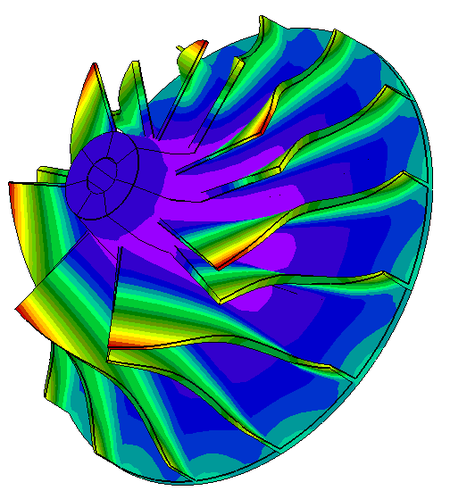
\includegraphics[width=.5\columnwidth]{fig/Lav.png}
	\caption{ターボチャージャーのコンプレッサー}
	\label{fig:001}
\end{figure}
%
\begin{table}[H]
	%\caption{}
	\label{tab:001}
	\centering
	\begin{tabular}{|l|l|}
		\hline
		原作者                     & Guido Dhondt氏、Klaus Wittig氏                          \\ \hline
		安定版リリース             & 2.17 / 2020年7月26日;10か月前                           \\ \hline
		リポジトリ                 & \href{https://github.com/calculix}{GitHub.com/calculix} \\ \hline
		オペレーティング・システム & Linux、Windows                                          \\ \hline
		種類                       & 有限要素解析                                            \\ \hline
		ライセンス                 & GPL(フリーソフトウェア)                               \\ \hline
		ウェブサイト               & \href{http://www.calculix.de/}{www.calculix.de}         \\ \hline
	\end{tabular}
\end{table}
%
\section{CalculiXとは}\label{sec:CalculiX}
%
\textbf{CalculiX}は、Abaqusと同様の入力形式を使用する、フリーでオープンソースの有限要素解析アプリケーションです。
Guido Dhondt氏が開発した陰解法および陽解法ソルバー(CCX)と、Klaus Wittig氏が開発したプリ・ポストプロセッサ(CGX)を備えています\footnote{\href{http://www.calculix.de/}{CalculiXのウェブサイト}}。
元のソフトウェアはLinux\footnote{\href{http://www.libremechanics.com/?q=node/9}{Ubuntu11.04以降でCalculiX2.6マルチスレッドをインストールする方法}}オペレーティング・システム用に書かれたものです。\footnote{\href{http://www.calculix.de/}{CalculiXのウェブサイト}}
Convergent Mechanical社は、アプリケーションをWindowsオペレーティングシステムに移植しました。\footnote{\href{http://www.bconverged.com/}{Convergent Mechanical社のWebサイト}}

CalculiXのプリプロセッサコンポーネントは、数値流体力学プログラムであるduns、ISAAC、OpenFOAM用のグリッドデータを生成できます。
また、商用FEMプログラムであるNastran、Ansys、Abaqusの入力データを生成することもできます。\footnote{\href{http://imechanica.org/node/1628}{iMechanicaによるCalculiXレビュー}}
プリプロセッサは、STLファイルからメッシュデータを生成することもできます。\footnote{\href{http://bconverged.com/calculix/doc/cgx/html/cgx.html}{CGXドキュメント}}

Yahoo!ディスカッショングループを通じてサポートを提供する活発なオンラインコミュニティが存在しました\footnote{CalculiX Yahoo!グループ}。
現在のディスカッショングループはDiscourseにあります。\footnote{\href{https://calculix.discourse.group/}{CalculiX Discourseグループ}}
Convergent Mechanical社は、Windows用CalculiXの拡張バージョンのインストールサポートも提供しています。\footnote{\href{http://www.bconverged.com/}{Convergent Mechanical社のWebサイト}}

WindowsとLinuxの両方に対応したCCXウィザードを備えた使いやすいCalculiX Launcher\footnote{\href{https://sourceforge.net/projects/calculixforwin/}{CalculiX Launcher(SourceForge)}}があります。\footnote{\href{http://calculixforwin.blogspot.mx/2015/05/calculix-launcher.html}{CalculiX Launcher}}

また、新しいLinuxサブシステムWSLを搭載したWindows 10 Fall Creator(1709)へのインストールも可能です\footnote{「\href{https://carlomonjaraztec.wordpress.com/2017/07/10/ccx_in_win10/}{元のソースからWindows Subsystem for inux(WSL)を使用してWindows10にCalculiXをインストールする方法}」(2017年7月10日)}。

CalculiXソルバーは、Sun Gridで利用可能です\footnote{Sun Gridに新しいアプリケーションが登場しました。
Calculix Archived 2007-05-28 at Wayback Machine、May 2007.}。

Pythonライブラリーpycalculix\footnote{\href{http://justinablack.com/pycalculix/}{pycalculixのウェブサイト}}は、Pythonプログラミング言語でCalculiXモデルの作成を自動化するために作成されました。
ライブラリは、2Dモデルの構築、読み込み、メッシュ生成、解法、およびCalculiXの結果の照会を行うためのPythonアクセスを提供します。
PycalculixはJustin Black氏によって書かれました。
例題やチュートリアルは、pycalculixのサイトで入手できます。

FreeCAD\footnote{\href{https://freecadweb.org/}{FreeCADのWebサイト}}は、Calculixモデルの作成を自動化するFEMワークベンチを開発しました。

ブランデンブルク応用科学大学のMartinKraska教授によるCalculiX\footnote{\href{https://github.com/mkraska/CalculiX-Examples/}{CalculiXの例題}}の良い使用例はたくさんあります。

\section{文献}\label{sec:Literature}

\begin{itemize}
	\item Guido Dhondt氏:「3次元熱機械的応用のための有限要素法」。Wiley、Hoboken 2004、ISBN 0-470-85752-8
	\item \href{http://bconverged.com/calculix/doc/ccx/html/ccx.html}{現在のCCXドキュメント}
	\item \href{http://bconverged.com/calculix/doc/cgx/html/cgx.html}{現在のCGXドキュメント}
	\item \href{http://www.bconverged.com/content/calculix/doc/GettingStarted.pdf}{スタートアップガイド}
	\item \href{https://freecadweb.org/wiki/FEM_Module}{CalCulix用FreeCAD FEMワークベンチ}
\end{itemize}

\section{外部リンク}\label{sec:References}

\begin{itemize}
	\item \href{http://www.calculix.de/}{公式ウェブサイト}
	\item \href{http://www.feacluster.com/calculix.php\#1}{検索可能なオンライン・ドキュメント}
	\item \href{http://bconverged.com/calculix}{CalculiX for Windows}
	\item CalculiXディスカッション・グループ
	\item \href{http://justinablack.com/pycalculix/}{pycalculixのウェブサイト}
	\item \href{https://forum.freecadweb.org/viewtopic.php?f=18\&t=12212}{FreeCAD FEMワークベンチ}
	\item \href{http://tfel.sourceforge.net/calculix.html}{CalculiX用MFrontコードジェネレーター}
\end{itemize}
\end{document}